\documentclass[conference]{IEEEtran}
\IEEEoverridecommandlockouts
\usepackage{amsmath,amssymb}
\usepackage{booktabs}
\usepackage{url}
\usepackage{tikz}
\usetikzlibrary{arrows.meta,positioning}

\begin{document}

\title{Riptide: Breaking the Serial Window Chain in\\ Parallel Gzip Decompression\\
\large Methodology Report}

\author{
\begin{tabular}{@{}c@{\hspace{2.2cm}}c@{}}
\textbf{Devansh Hiren Shah} & \textbf{Mantri Samarth Prakash}\\
Dept. of Information Technology & Dept. of Information Technology\\
NIT Karnataka, Surathkal --- 241IT024 & NIT Karnataka, Surathkal --- 241IT043\\[8pt]
\textbf{Shubh Minesh Thakkar} & \textbf{Ritesh Bhagat}\\
Dept. of Information Technology & Dept. of Information Technology\\
NIT Karnataka, Surathkal --- 241IT076 & NIT Karnataka, Surathkal --- 241IT063
\end{tabular}
}

\maketitle

\section{Methodology}

Our base paper is \texttt{rapidgzip}~\cite{rapidgzip}, which decodes unmodified
gzip files in parallel using the two-stage scheme introduced by
\texttt{pugz}~\cite{pugz}. Each thread decodes a chunk of the stream without
knowing the 32\,KiB window that precedes it, writing placeholders (markers) for
the unknown bytes, and the markers are replaced once the window is known. The
windows themselves are obtained one chunk after another: the base paper states
that this propagation cannot be parallelised, and attributes to it an Amdahl
bound on scaling. Without an index, its measured throughput stops scaling at
about 64 cores on Silesia and 48 cores on FASTQ data, whereas the index path,
which has no markers to resolve, scales to 128 cores~\cite{rapidgzip}.

Our primary contribution parallelises that step. We also address the base
paper's handling of chunks with very high compression ratios, which it lists as
future work. Both are implemented as changes to the base paper's open-source code
(MIT/Apache-2.0), so that every comparison is between the two systems at the
same commit.

\subsection{Dataset}

\emph{Nature of the data.} The data is a corpus of compressed streams rather than
a labelled learning dataset. Each item is an unmodified \texttt{.gz} file paired
with the output of \texttt{zlib}, which serves as ground truth: a result is
correct only if it matches that output byte for byte.

\emph{Instances and features.} The unit of analysis is one DEFLATE
block~\cite{deflate}. For every block we record its start offset in bits, input
size in bits, output size in bytes, block type (stored, fixed- or
dynamic-Huffman), and its counts of literal and match symbols; per file we record
match-distance and match-length histograms. From these we derive the per-block
expansion ratio $\rho = \text{output bytes}/\text{input bytes}$ and, for every
chunk, the fraction of its final window that is still unresolved, which is what
the window chain must propagate.

\emph{Silesia corpus.} Our primary dataset is the Silesia corpus, the benchmark
the base paper uses. We obtained it from its maintainer's distribution
(12 files, 212\,MB), compressed each file with \texttt{gzip} at its default
level, and built a tarball of all twelve, as the base paper does. The tarball is
68.2\,MB and expands 3.11$\times$, matching the 3.1$\times$ the base paper
reports. We wrote a reference DEFLATE decoder that records every block boundary;
it is an offline measurement tool, not a stage of the parallel decoder. It
decoded all twelve files and the tarball bit-identically to \texttt{zlib}.
Table~\ref{tab:silesia} gives per-file statistics. The corpus spans a
7.7$\times$ range of compression ratios, from 1.36 (\texttt{sao}) to 10.48
(\texttt{nci}), inside a single archive.

\begin{table}[t]
\caption{Silesia corpus statistics (measured)}
\label{tab:silesia}
\centering
\footnotesize
\setlength{\tabcolsep}{3pt}
\begin{tabular}{@{}llrrrr@{}}
\toprule
\textbf{File} & \textbf{Content} & \textbf{Out MiB} & \textbf{Ratio} & \textbf{Blocks} & $\boldsymbol{\rho}$ \textbf{mean $\pm$ sd} \\
\midrule
\texttt{dickens} & English text      &  9.72 &  2.63 & 127 &  2.63 $\pm$ 0.05 \\
\texttt{mozilla} & Executables (tar) & 48.85 &  2.68 & 870 &  2.58 $\pm$ 1.31 \\
\texttt{mr}      & MRI image         &  9.51 &  2.71 & 140 &  2.69 $\pm$ 0.68 \\
\texttt{nci}     & Chemical database & 32.00 & 10.48 & 109 & 10.44 $\pm$ 1.67 \\
\texttt{ooffice} & Office DLLs       &  5.87 &  1.99 & 136 &  2.00 $\pm$ 0.64 \\
\texttt{osdb}    & Database          &  9.62 &  2.73 & 169 &  2.73 $\pm$ 0.04 \\
\texttt{reymont} & Polish text (PDF) &  6.32 &  3.56 &  62 &  3.53 $\pm$ 0.41 \\
\texttt{samba}   & Source code (tar) & 20.61 &  3.96 & 227 &  3.57 $\pm$ 2.19 \\
\texttt{sao}     & Star catalogue    &  6.92 &  1.36 & 260 &  1.36 $\pm$ 0.03 \\
\texttt{webster} & Dictionary        & 39.54 &  3.39 & 415 &  3.39 $\pm$ 0.18 \\
\texttt{x-ray}   & X-ray image       &  8.08 &  1.40 & 278 &  1.40 $\pm$ 0.04 \\
\texttt{xml}     & XML               &  5.10 &  7.77 &  24 &  7.41 $\pm$ 5.94 \\
\midrule
Tarball          & All twelve        & 202.14 & 3.11 & 2{,}811 & \\
\bottomrule
\end{tabular}
\end{table}

Table~\ref{tab:snapshot} shows a snapshot of the block records at the boundary
between \texttt{nci} and \texttt{ooffice} inside the tarball. Blocks of similar
compressed size fall from about 255\,KB of output to about 41\,KB, so a chunk
cut by compressed size can need several times more memory than its neighbour
while costing a similar number of symbol decodes.

\begin{table}[t]
\caption{Snapshot of block records, Silesia tarball (\texttt{nci} $\rightarrow$ \texttt{ooffice})}
\label{tab:snapshot}
\centering
\footnotesize
\setlength{\tabcolsep}{3pt}
\begin{tabular}{@{}rlrrrrr@{}}
\toprule
\textbf{\#} & \textbf{Type} & \textbf{In bits} & \textbf{Out B} & \textbf{Literals} & \textbf{Matches} & $\boldsymbol{\rho}$ \\
\midrule
1242 & dynamic & 228{,}422 & 255{,}724 &  7{,}195 & 9{,}188 & 8.96 \\
1243 & dynamic & 228{,}542 & 250{,}915 &  7{,}055 & 9{,}328 & 8.78 \\
1244 & dynamic & 188{,}734 &  89{,}461 & 10{,}666 & 5{,}717 & 3.79 \\
1245 & dynamic & 181{,}854 &  40{,}749 & 11{,}285 & 5{,}098 & 1.79 \\
1246 & dynamic & 184{,}028 &  42{,}317 & 11{,}156 & 5{,}227 & 1.84 \\
\bottomrule
\end{tabular}
\end{table}

The full evaluation adds public \texttt{.fastq.gz} reads (the base paper's
weakest-scaling case), gzipped logs and CSV exports, data compressed above
20$\times$, and a synthetic class authored by us that covers legal but rare
encodings: stored and fixed-Huffman blocks, empty blocks, overlapping copies with
$\ell > d$, maximum-distance references, single-block files, and truncated or
bit-flipped streams. Runtime experiments use files of at least 1\,GB, built where
necessary by concatenating copies as the base paper does.

\emph{Preprocessing.} Each stream is (i)~decompressed with \texttt{zlib}, with
failing files routed to the error-path set and the SHA-256 of valid outputs
stored as ground truth; (ii)~classified as single- or multi-member, since
multi-member files are trivially splittable and are reported separately;
(iii)~profiled offline to produce block records; and (iv)~bucketed by size, by
the dispersion of $\rho$, and by the unresolved-window fraction. Bytes are never
altered, as format fidelity on unmodified input is a constraint of the problem.

\subsection{Proposed Method}

Fig.~\ref{fig:block} shows the pipeline. Bold-outlined stages are our
contributions; the remaining stages are inherited from the base paper and are
not claimed as novel.

\begin{figure*}[t]
\centering
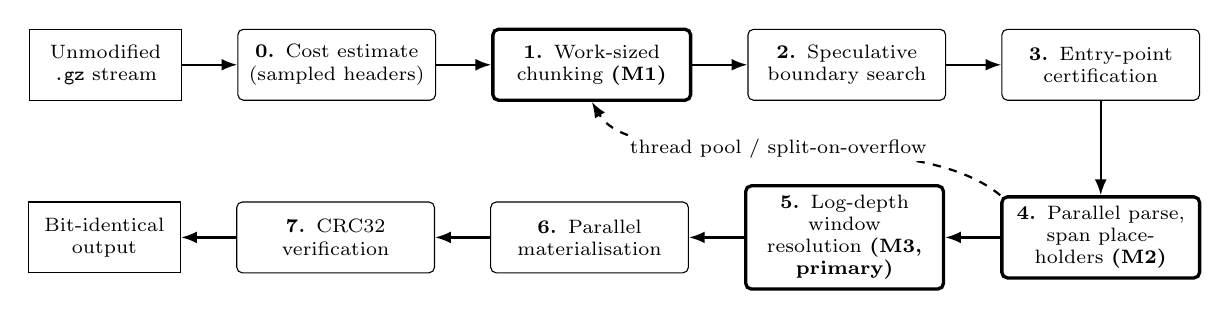
\begin{tikzpicture}[
  node distance=6mm and 7mm,
  box/.style={draw, rounded corners=2pt, align=center, font=\scriptsize,
              minimum height=9mm, inner xsep=3pt, text width=23mm},
  novel/.style={box, very thick},
  io/.style={draw, align=center, font=\scriptsize, minimum height=9mm,
             text width=17mm},
  a/.style={-{Latex[length=2mm]}, thick}
]
\node[io] (in) {Unmodified\\ \texttt{.gz} stream};
\node[box, right=of in]      (prof) {\textbf{0.} Cost estimate\\ (sampled headers)};
\node[novel, right=of prof]  (part) {\textbf{1.} Work-sized\\ chunking \textbf{(M1)}};
\node[box, right=of part]    (b1)   {\textbf{2.} Speculative\\ boundary search};
\node[box, right=of b1]      (b2)   {\textbf{3.} Entry-point\\ certification};
\node[novel, below=12mm of b2]  (parse) {\textbf{4.} Parallel parse,\\ span placeholders \textbf{(M2)}};
\node[novel, left=of parse]     (res)   {\textbf{5.} Log-depth window\\ resolution \textbf{(M3, primary)}};
\node[box, left=of res]         (mat)   {\textbf{6.} Parallel\\ materialisation};
\node[box, left=of mat]         (crc)   {\textbf{7.} CRC32\\ verification};
\node[io, left=of crc]          (out)   {Bit-identical\\ output};
\draw[a] (in) -- (prof);
\draw[a] (prof) -- (part);
\draw[a] (part) -- (b1);
\draw[a] (b1) -- (b2);
\draw[a] (b2.south) -- (parse.north);
\draw[a] (parse) -- (res);
\draw[a] (res) -- (mat);
\draw[a] (mat) -- (crc);
\draw[a] (crc) -- (out);
\draw[a, dashed] (parse.north west) .. controls +(-1.2,1.0) and +(0.6,-1.0) ..
   node[midway, font=\scriptsize, fill=white, inner sep=1pt]
   {thread pool / split-on-overflow} (part.south);
\end{tikzpicture}
\caption{Proposed pipeline. Contributions: log-depth window resolution by
prefix scan (M3, primary), work-sized chunking with parallel splitting of
oversized chunks (M1), and span placeholders (M2, supporting). Boundary search,
entry-point certification, materialisation within a chunk, and parallel CRC32
verification are inherited from the base paper. The dashed edge is the runtime
path by which a chunk that exceeds its output budget is split and returned to the
thread pool.}
\label{fig:block}
\end{figure*}

\emph{Inherited foundation.} Reading compressed bits into symbols depends only on
the current block's Huffman tables and bit position; only executing a
back-reference needs earlier output. A chunk can therefore be decoded before its
predecessor, writing for each unknown byte a marker $256 + j$ meaning ``byte $j$
of the 32\,KiB window preceding this chunk''~\cite{pugz}. Candidate block starts
are found by a speculative block finder and confirmed by successful
decoding~\cite{rapidgzip}.

\emph{M3 (primary): window resolution by parallel prefix scan.} Let $W_k$ be the
32\,KiB window at the end of chunk $k$. After first-stage decoding, every entry of
chunk $k$'s final window is either a known byte or a marker into $W_{k-1}$, so the
window is a map $f_k$ with $W_k = f_k(W_{k-1})$. The base paper evaluates this
chain sequentially, one chunk at a time. The composition of two such maps is
again a map of the same form, a known byte or an index into an earlier window,
and composition is associative. The chain is therefore a prefix computation,
\[
W_k = (f_k \circ f_{k-1} \circ \cdots \circ f_1)(W_0),
\]
which a parallel prefix scan evaluates in $\lceil \log_2 N \rceil$ rounds for $N$
chunks instead of $N-1$ dependent steps. Each composition is a gather over
32\,KiB, the same operation as marker replacement. We use a work-efficient
(Blelloch) scan, giving $O(NW)$ work and $O(W \log N)$ span for window size $W$,
applied to each batch of prefetched chunks and seeded with the last resolved
window.

We prototyped M3 on the Silesia tarball, cutting chunks the way the base paper
does: a chunk starts at the first block at or after each multiple of the chunk
size in the compressed stream. Every chunk was decoded independently from an
unknown window, and the windows were resolved both sequentially and by scan
(Table~\ref{tab:scan}). At both chunk sizes the scan's windows were identical to
the sequential chain's and the final output was bit-identical to \texttt{zlib}.

\begin{table}[t]
\caption{Prototype of M3 on the Silesia tarball}
\label{tab:scan}
\centering
\footnotesize
\setlength{\tabcolsep}{4pt}
\begin{tabular}{@{}lrr@{}}
\toprule
\textbf{Chunk size (compressed)} & \textbf{4\,MiB} & \textbf{512\,KiB} \\
\midrule
Chunks $N$ & 17 & 131 \\
Sequential steps / scan rounds & 16 / 5 & 130 / 8 \\
Windows identical, output bit-identical & yes & yes \\
Final windows still containing markers & 18.8\% & 67.7\% \\
Chunk output held in 16-bit form & 38.7\% & 78.1\% \\
Serial chain, share of resolution work & 0.25\% & 2.0\% \\
\bottomrule
\end{tabular}
\end{table}

The table also bounds what M3 can gain. The chain's share of marker-resolution
work grows eightfold as chunks shrink from 4\,MiB to 512\,KiB, but it remains
small in absolute terms: if resolution costs about a tenth of first-stage
decoding, as the base paper reports, the chain is about 0.2\% of total work even
at 512\,KiB. By that arithmetic alone the chain would not explain the base
paper's 64-core plateau, so either its serial step costs much more in practice
than a 32\,KiB gather (for example through in-order waiting and bookkeeping on
the coordinating thread), or the plateau has other causes as well. Measuring the
cost of that step inside the base paper's code is therefore the first task of
the implementation phase, and the size of M3's speedup is stated only after it.

\emph{M1 (secondary): work-sized chunking with parallel splitting.} The base
paper's first pass cuts chunks by compressed size and relies on its thread pool
for balance; it balances by decompressed size only when an index already exists,
and it lists splitting chunks with very high compression ratios as future
work~\cite{rapidgzip}. The released software instead caps each chunk's output,
which serialises decoding above about $20\times$ compression~\cite{changelog}.
M1 sizes chunks from a cost estimate taken from sampled block headers and, when
a chunk exceeds its output budget, splits the remainder at a block boundary and
hands the pieces to idle workers, keeping the memory bound without serialising.
On the Silesia block records, a thread-pool model with an oracle that knows every
block's true cost gives a load-imbalance factor $\lambda = T_{\max}/\bar{T}$ of
1.00 for work-sized chunks against 1.16 for compressed-size chunks with 8 workers
and four chunks each, and 1.01 against 1.20 with 16 workers. These are upper
bounds on what M1 can gain, not measurements.

\emph{M2 (supporting): compact spans.} Markers widen output to 16 bits until a
chunk's window becomes marker-free, after which the base paper's software
switches to 8-bit decoding~\cite{rapidgzip}. On Silesia this widened region is
38.7\% of each chunk at 4\,MiB but 78.1\% at 512\,KiB (Table~\ref{tab:scan}), so
it dominates exactly when chunks are made small to save memory. M2 keeps output
at 8 bits and records each unresolved run as a span
$(\textit{dst}, \textit{win\_off}, \textit{len})$, so that the composed window maps
of M3 apply to runs rather than to individual bytes.

\emph{Verification.} Parallel CRC32 verification by combining per-chunk checksums
is already part of the base paper's software~\cite{changelog} and is reused, not
claimed.

\subsection{Evaluation Metrics, Experimental Settings, and Expected Analysis}

\emph{Metrics.} Correctness is a gate: a configuration is admissible only if its
output is byte-identical to \texttt{zlib} on every file and it rejects every
malformed stream at the same offset. For M3 we measure the time the base paper's
code and ours spend propagating windows, against $\lceil \log_2 N \rceil$ rounds,
and the core count at which throughput stops scaling as a function of chunk
size. Overall performance is throughput (MB/s of output), speedup
$S_P = T_1/T_P$ and efficiency $E_P = S_P/P$. Cold-start time is total wall time
on first access with no index, including the cost estimate, so that M1 cannot
hide its own overhead; single-thread Riptide time is divided by \texttt{igzip}
time so that speedup is also reported against the best sequential decoder. M1 is
measured by $\lambda$, and M2 by peak resident memory divided by output size.

\emph{Experimental settings.} Experiments run on a single multicore node whose
core count, cache hierarchy, memory capacity and bandwidth, compiler and library
versions are reported. Baselines are \texttt{zlib}, \texttt{igzip}, \texttt{pigz}
and \texttt{rapidgzip} built from the same commit our changes are applied to.
The first experiment instruments that build to time its serial window
propagation on Silesia. Chunk size is varied over $\{0.5, 1, 2, 4\}$\,MiB, since
Table~\ref{tab:scan} shows the chain's share growing as chunks shrink; thread
count is varied over $P \in \{1, 2, 4, 8, 16, 32\}$ subject to available cores;
and cache state is cold (page cache dropped) or warm. Each configuration runs 10
times and medians with interquartile ranges are reported. Paired per-file timings
are compared with the Wilcoxon signed-rank test at $\alpha = 0.05$ with
Holm--Bonferroni correction, and effect sizes are reported. M1, M2 and M3 are
toggled independently, giving eight ablation configurations.

\emph{Expected analysis.} We state these predictions in advance so that they can
fail.
\begin{enumerate}
\item The time the base paper's code spends in serial window propagation will
grow as chunks shrink, in line with Table~\ref{tab:scan}. If it is close to the
pure-work estimate, M3's end-to-end gain will be small and confined to many cores
and small chunks, and we will report it as such.
\item Where propagation is a measurable share of runtime, M3 will make it grow
with $\log N$ rather than $N$ and move the scaling knee to higher core counts,
most on back-reference-heavy data such as Silesia and FASTQ.
\item M2 will reduce peak memory most at small chunk sizes, where most of each
chunk is held in 16-bit form.
\item On heterogeneous archives, M1 will keep $\lambda$ near 1 with few chunks per
worker. If measured $\lambda$ for compressed-size chunks is already near 1, M1
will be reported as a negative result.
\end{enumerate}
Results will be interpreted in that order: correctness first, then the measured
cost of the serial step, then whether each mechanism removes the limitation it
targets.

\begin{thebibliography}{00}
\bibitem{rapidgzip} M. Knespel and H. Brunst, ``Rapidgzip: Parallel decompression and seeking in gzip files using cache prefetching,'' in \emph{Proc. 32nd Int. Symp. High-Performance Parallel and Distributed Computing (HPDC '23)}, Orlando, FL, USA, 2023, doi: 10.1145/3588195.3592992.
\bibitem{pugz} M. Kerbiriou and R. Chikhi, ``Parallel decompression of gzip-compressed files and random access to DNA sequences,'' in \emph{Proc. IEEE Int. Parallel and Distributed Processing Symp. Workshops (IPDPSW)}, 2019, pp. 209--217, doi: 10.1109/IPDPSW.2019.00042.
\bibitem{deflate} P. Deutsch, ``DEFLATE compressed data format specification version 1.3,'' RFC 1951, 1996, doi: 10.17487/RFC1951.
\bibitem{changelog} M. Knespel, ``rapidgzip changelog,'' versions 0.6.0--0.16.0, 2023--2025. [Online]. Available: \url{https://github.com/mxmlnkn/rapidgzip/blob/main/CHANGELOG.md}
\end{thebibliography}

\end{document}
